%!TEX root = ../dokumentation.tex

\chapter{Umsetzung}\label{cha:Umsetzung}
<Allgemeine Beschreibung des Inhalts des Kapitels.>

\section{Infrastruktur \& Prozesse}
Vor Beginn der Entwicklung werden im folgenden die Umgebung, in welcher die Applikation später ausgeführt werden soll, sowie der Anwendungsprozess, genauer definiert. 

<Weitere Einführung in das Kapitel bzw. aktuelle überarbeiten>

\subsection{Beschreibung der Infrastruktur}
<...Einleitung/überleitung zur beschreibung der infrastruktur>

Alle Server (sowohl Wen- wie auch Application-Server), schreiben ihre jeweiligen Logfiles auf ein \ac{NFS}. Der entsprechende Infrastruktur-Server mounted die benötigten Verzeichnisse. Der Server verfügt über eine Hadoop Installation, auf welcher die Applikation ausgeführt wird (siehe \autoref{fig:AufbauInfrastruktur}).

\begin{figure}
	\centering
	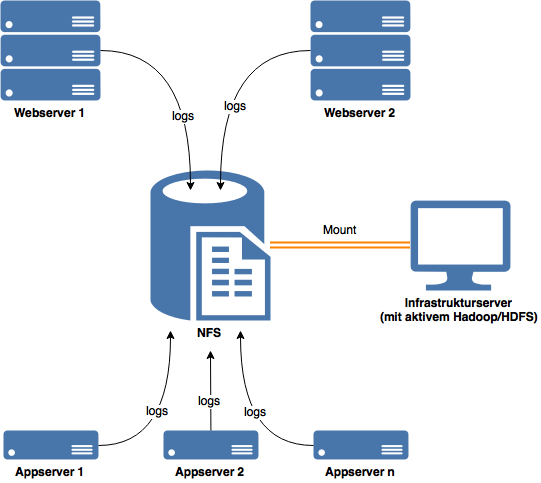
\includegraphics[width=.8\textwidth]{Infrastruktur.png}
	\caption{DUMMY: Aufbau der Infrastruktur}
	\label{fig:AufbauInfrastruktur}
\end{figure}

\subsection{Definition des Anwendungsprozesses}


\begin{figure}
	\centering
	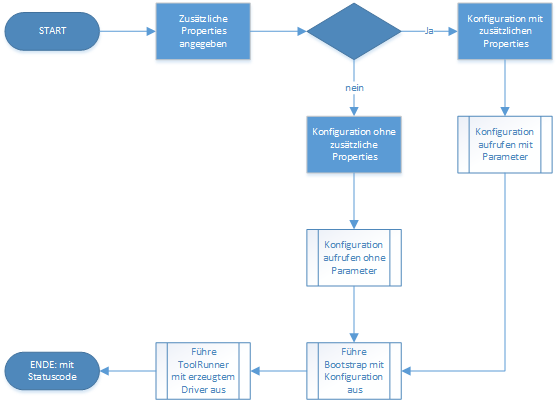
\includegraphics[scale=1]{PAP_Main_main.png}
	\caption{PAP für main Methode der Main Klasse}
	\label{fig:PAP_Main_main}
\end{figure}

<Hier sollte der Prozess der Anwendung geplant werden. wo liegen die Daten? wie findet der zugriff statt? nach welchem schema sind sie abgelegt und benannt? Außerdem sollte klar werden wie die Informationen verarbeitet werden. ein großer map reduce oder eine verkettung mehrerer mapper und reducer? Außerdem muss das ausgabeformat festgelegt werden. Bzw. zwei alternativen. eine für wenn die anwendung performant genug ist um als check skript zu laufen, und eine für den fall das nicht.>

\section{Die Konfigurationsschnittstelle}
Wie bereits bei der Beschreibung des Verarbeitungsprozesses gezeigt wurde, wird direkt nach dem Start der Anwendung eine Initialisierung vorgenommen. Hierbei soll die Umgebung so konfiguriert werden, dass die gewünschte Analyse durch die Anwendung ohne Probleme vorgenommen werden kann.

Die Konfiguration der Anwendung wird durch Dateien vom Typ \textit{.properties} vorgenommen. Diese werden von Java vollständig unterstützt. Für die Interpretation der Konfigurationsdateien wird auf die Klasse \textit{java.util.Properties} zurückgegriffen. Die Funktionsweise der Properties wird im folgenden genauer betrachtet.

\subsection{Aufbau von Properties}
Die Konfigurationswerte werden in Properties Dateien als Schlüssel-Wert-Paare gespeichert. Die Trennung kann hierbei durch einen Doppelpunkt oder Gleichheitszeichen erfolgen. Des weiteren ist es möglich, Platzhalter bei den Werten zu definieren, welche später durch Variablen ersetzt werden können. Außerdem ist es möglich, zum besseren Verständnis, die Datei um Kommentare zu erweitern. Jede Zeile, welche mit einem Hash oder Ausrufezeichen beginnt, wird als Kommentar gesehen, und von der Anwendung nicht interpretiert. \autoref{lis:AuszugDefaultProperties} zeigt einen Auszug aus der \textit{default.properties} Datei. \\

\begin{lstlisting}[language=Bash,caption=Auszug aus default.properties,label=lis:AuszugDefaultProperties]
###
# Default properties for Logfileanalyzer.
# Properties can be extended by user defined properties.
# Never change this file to fit one case.
#

# Set mode for execution (DEBUG, TEST, LIVE)
RUNMODE         : DEBUG

# Runtime properties
LOGTARGET       : {0}

[...]
\end{lstlisting}

Grundsätzlich sind alle Konfigurationen vom Typ \textit{String}. Es ist, nativ, nicht möglich, direkt einen Wert in einem anderen Datentyp zu definieren. Falls eine Typenkonvertieren notwendig ist, muss diese manuell durchgeführt werden.

In Java stellt die Klasse \textit{Properties}, welche teil des \textit{java.util} Paketes ist, alle benötigten Methoden bereit. Um die Konfiguration der Anwendung zu vereinfachen, wurde die Klasse \textit{Configuration} im Paket \textit{com.hszuesz.logfileanalyzer} erzeugt. Diese leitet sich aus der Klasse \textit{Properties} ab, und stellt Erweiterungen zum einlesen mehrerer Konfigurationsdateien bereit. Dies ist notwendig, um eine stufenweise Konfiguration der Anwendung zu realisieren.

Da die Anwendung später innerhalb des Hadoop Frameworks ausgeführt wird, müssen die Konfigurationsdateien ein Teil der, durch Maven erzeugten, JAR-Datei sein. Dies wird durch eine Ergänzung in der \textit{pom.xml} innerhalb des \textit{build} Knotens sichergestellt (siehe \autoref{lis:POMErgänzung}). \\

\begin{lstlisting}[language=XML,caption=pom.xml Ergänzung für Konfigurationsdateien,label=lis:POMErgänzung]
[...]
	<resources>
		<resource>
			<directory>conf</directory>
			<includes>
				<include>*.properties</include>
			</includes>
		</resource>
	</resources>
[...]
\end{lstlisting}

\subsection{Beschreibung der Konfigurationsstufen}
Die Konfiguration der Anwendung wird in drei Stufen durchgeführt. Dies soll die Komplexität der Konfigurationsdateien reduzieren, indem die individuellen Anpassungen für jede Ausführung des Programms gekapselt, und immer gleiche Einstellungen ausgelagert werden.

Die erste Stufe bilden die sog. Core-Properties, welche in der Datei \textit{core.properties} hinterlegt sind. Wie der Name bereits erkennen lässt, handelt es sich hierbei um Grundlegende Einstellungen, welche den Kern der Anwendung beeinflussen. Dazu gehört z.B. die Konfiguration der verschiedenen \textit{RUNMODES} oder Pfade zu weiteren wichtigen Dateien, wie den Default- oder Logger-Properties. Ein überschreiben dieser Einstellungen ist nicht möglich.

Die zweite Stufe bildet die Defaults. Hier werden alle Konfigurationen vorgenommen, welche für eine Standardausführung der Anwendung benötigt werden. Alle Einstellungen, welche in der \textit{defaults.properties} Datei hinterlegt sind, können durch den Anwender verändert werden.

Die dritte und letzte Stufe bilden die User-Properties. Beim Start der Anwendung kann der Pfad zu einer individuellen Properties-Datei übergeben werden. In dieser können die Einstellungen, welche durch die Defaults vorgenommen wurden, ergänzt und  überschreiben werden.

Der Prozess für die Verarbeitung der einzelnen Stufen wird im \ac{PAP} der \textit{LFAConfiguration} verdeutlicht, welcher im Anhang zu finden ist.

%<Beschreibung wie Properties programmiert werden. Wie werden diese in der Anwendung umgesetzt? Welche Rolle spielen Properties für den generischen Teil der Anwendung?>

\subsection{Logger Konfiguration}
<Beschreibung wie der Logger in Java funktioniert und wie dieser hier eingesetzt wird. Speziell die Konfiguration über die logger.properties datei hervorheben.>

%\section{Grundlagen für Datenverarbeitung}
%<Beschreibung der Entwicklung für die Grundlagen zur Datenverarbeitung. Welche Klassen werden dabei verwendet? Welches System liegt dahinter? Warum dieses System? Dabei nicht nur auf die Speicherung von Daten eingehen sondern auch auf das Lesen von Dateien.>

\section{Bestimmung des Aufbaus der Logfiles}
<Wie sehen die Logfiles aus? Welche Formate haben sie? Welche rolle spielen diese bei der Datenverarbeitung? Welche Informationen sind die richtigen Informationen?>

\section{Implementierung von MapReduce}
Nachdem alle Grundlagen der Anwendung fertiggestellt wurden kann mit der Entwicklung des Kernstückes begonnen werden, der Implementierung von MapReduce. Dabei besteht die größte Hürde im generischen Ansatz, welcher, insbesondere im Kern des Programms, immer berücksichtigt werden muss.



\subsection{Einblick in die InputFormat Klasse}


\subsection{Der RecordReader}


\subsection{Mapper und Reducer}

<Beschreibung vom Kern der Anwendung. Wie wird der Algorithmus umgesetzt? Welche Klassen/Methoden sind notwendig? Wie unterscheidet sich die Implementierung bei unterschiedlichem Input. Spielt das überhaupt eine Rolle oder muss es nur Text sein? Welches Ergebnis bekommt man und in welcher Form?>

\section{Ausführungsdatei Logfileanalyzer.sh}

\begin{lstlisting}[language=Bash,caption=Ausführungsdatei Logfileanalyzer.sh,label=lis:Logfileanalyzer.sh]
#!/bin/bash

#Load config
. $1/config.cfg
#Cleanup input direktory on dfs
/bin/hdfs dfs -rm -r -skipTrash input/*
#Delete output directory on dfs
/bin/hdfs dfs -rm -r -skipTrash output
#Put input files on dfs
/bin/hdfs dfs -put $MAP_REDUCE_INPUT input
mkdir $MAP_REDUCE_OUTPUT
if [ $MAP_REDUCE_USE_USER_PROPERTIES == true ]
then
        #Export HADOOP_OPTS to pass user properties file
        export HADOOP_OPTS="-Dlfa.userconf=$1/$MAP_REDUCE_USER_PROPERTIES"
fi
if [ $MAP_REDUCE_USE_LOG == true ]
then
        #Use log logfile
        echo "Log file wird verwendet"
        /bin/hadoop jar $1/$MAP_REDUCE_JAR $MAP_REDUCE_MAIN input output 2> $MAP_REDUCE_LOGFILE
else
        echo "Kein Logfile"
        /bin/hadoop jar $1/$MAP_REDUCE_JAR $MAP_REDUCE_MAIN input output
fi
if [ $MAP_REDUCE_USE_USER_PROPERTIES == true ]
then
        #Unset HADOOP_OPTS after apllication finished
        export HADOOP_OPTS=""
fi
#Get output from dfs
/bin/hdfs dfs -get output/* $MAP_REDUCE_OUTPUT
if [ $MAP_REDUCE_DISPLAY_OUTPUT == true ]
then
        cat ${MAP_REDUCE_OUTPUT}/*
fi
\end{lstlisting}

<Beschreiben der Bash Datei, durch welche der job (Jar) ausgeführt wird. Beschreiben der einzlenen Schritte und der configuration>

\section{Anwendungstest \& Ergebnisse}

\begin{lstlisting}[language=Java,caption=Properties für Anwendungstest,label=lis:PropertiesAnwendungstest]
lfa.runmode              : DEBUG

lfa.driver.mapper        : com.hszuesz.logfileanalyzer.mapper.PatternMapper
lfa.driver.reducer       : com.hszuesz.logfileanalyzer.reducer.CountReducer

lfa.driver.input.format  : org.apache.hadoop.mapreduce.lib.input.TextInputFormat

lfa.driver.output.key    : org.apache.hadoop.io.Text
lfa.driver.output.value  : org.apache.hadoop.io.IntWritable
lfa.driver.output.format : org.apache.hadoop.mapreduce.lib.output.TextOutputFormat

lfa.driver.job.name      : Laufzeittest webadapter.log

lfa.mapper.pattern.key   : \\] ([A-Z]{4,5})
lfa.mapper.nomatchaction : SKIP
\end{lstlisting}

\begin{figure}
	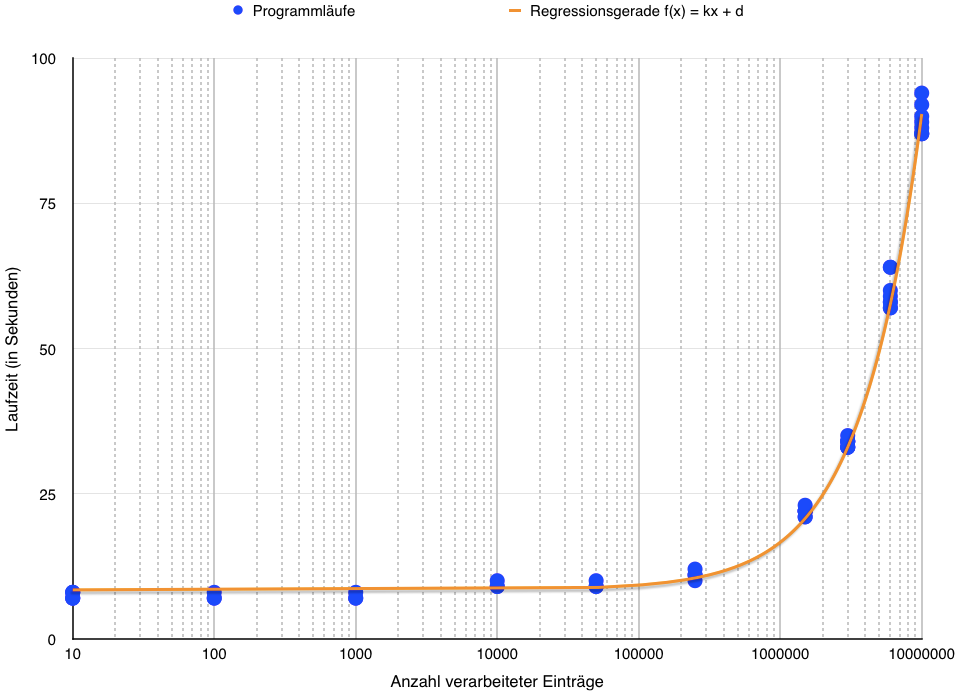
\includegraphics[width=1\textwidth]{Laufzeitanalyse.png}
	\caption{Laufzeitanalyse für Logfileanalyzer}
	\label{fig:Laufzeitanalyse}
\end{figure}

\begin{align}
f_1(x) &= 8,199 \times 10^{-6} x + 8,418 \label{equ:Laufzeit} \\
f_2(x) &= f_1(x) \times 5 \label{equ:MaxInterval}
\end{align}
<IDEE: Es wurde eine formel angegeben, welche aussage über die maximale ausführungsdauer gibt...eventuell lassen sich diese beiden formeln verbinden (also eine Formel die aussage gibt über den maximal möglichen intervall für eine bestimmte datenmenge \autoref{equ:MaxInterval})>

\begin{figure}
	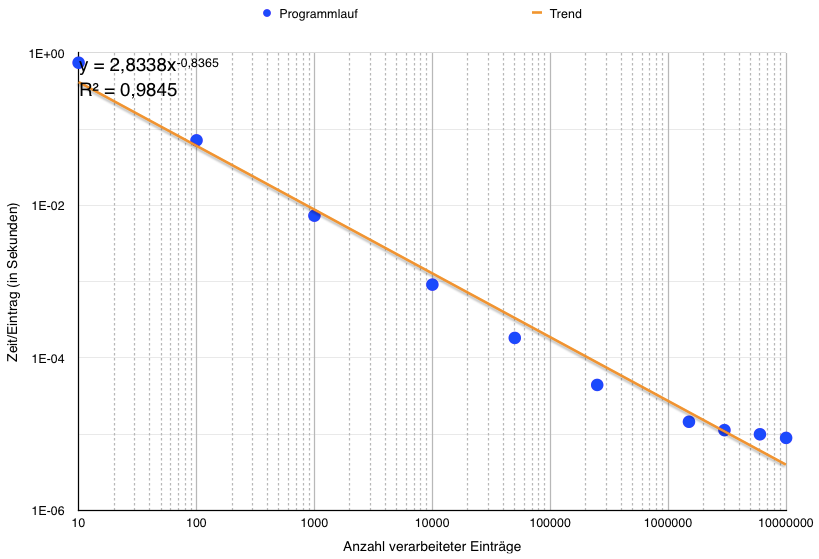
\includegraphics[width=1\textwidth]{Zeit_Pro_Eintrag.png}
	\caption{Verarbeitungszeit pro Eintrag}
	\label{fig:VerarbeitungszeitProEintrag}
\end{figure}

<Dokumentation der Tests mit unterschiedlich großen Datenmengen (10 Logeinträge bis 10.000.000 Einträge). Grafische Darstellung der Laufzeiten. Jede Stufe min. 10 mal ausführen und Ausführungszeit Nottieren/Dokumentieren. In Kapitel 6 Erkenntnisse aus den Tests aufarbeiten>